
%\subsection{3D Enviroment Specifics}
\section{Implementation}

\subsection{Algorithm}
\label{ss:algorithm}

The simulation follow the ray tracing technique outlined by
\citet{bell1997simulation} for side scan sonar, but applies it to a forward
looking sonar imaging sonar (section \ref{ss:avaible_models}). It also uses a
noising adding step as suggested by \citet{coiras2009gpu} with statistics
provided by \citet{maussang2007mean}.
No movement induced distortion was considered, some approachs to add this
feature is available on \citet{bell1999techniques,borawski2005sonar}. Also,
spreading and absorption losses are ignored, assuming they are compensated by
TVG (see section \ref{sss:tvg}).

Sonar parameters follow a Tritech's Micron sonar\cite{micronsonar}
information as output power, dynamic gain, beam step and sensibility were found
on official Tritech's documentation\cite{micronsonar,micronmodem}. The directional
gain was measured by the National Physical Laboratory, UK.

Simulation's output is, just as on the sonar, a sequence of arrays with values
between 0 and 255. Each element of the sequence is a bearing, direction of the
emitted sound pulse, and the array's components are the bins' values, sound
intensity received at some range of distances (calculated from echo delay).

\begin{figure}[h]
	\centering
	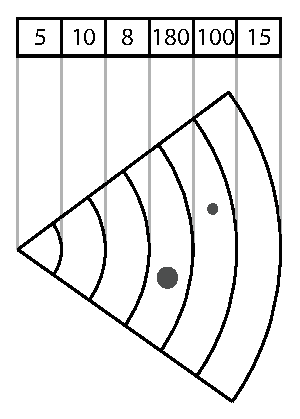
\includegraphics[scale=1.,clip]{Chap2/fig/sonarresponse.eps}
	\caption{Exemple of an array for a bearing direction. Actual arrays are
	longer, depending on resolution.}
	\label{fig:bins}
\end{figure}

The algorithm implementation uses the programming language Python with the
mathematical library NumPy, specially for efficient linear algebra. Most of the
treatment uses linear algebra to treat batch of rays at once.

\begin{figure}[ht]
    \centering
    \subfloat[Sonar Loop]{{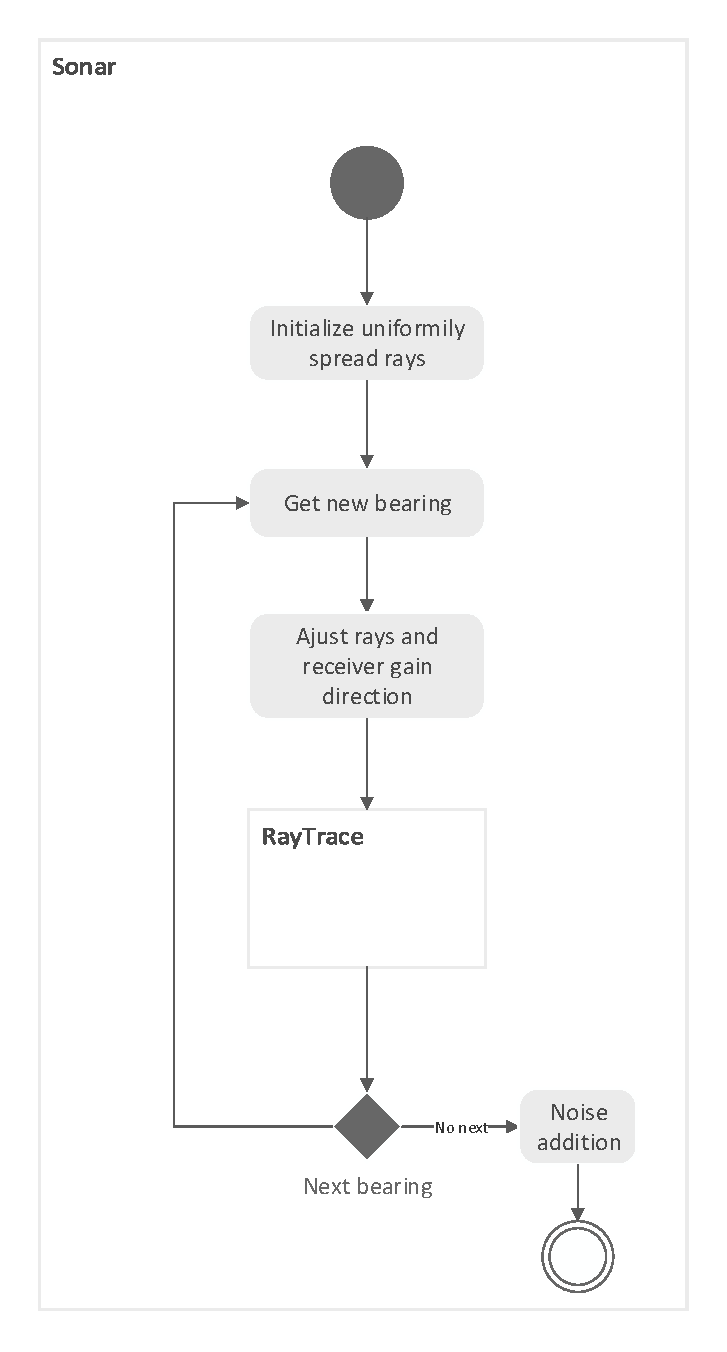
\includegraphics[width=75mm]{Chap2/fig/sonarflow}}}%
    \hfill
    \subfloat[RayTracer]{{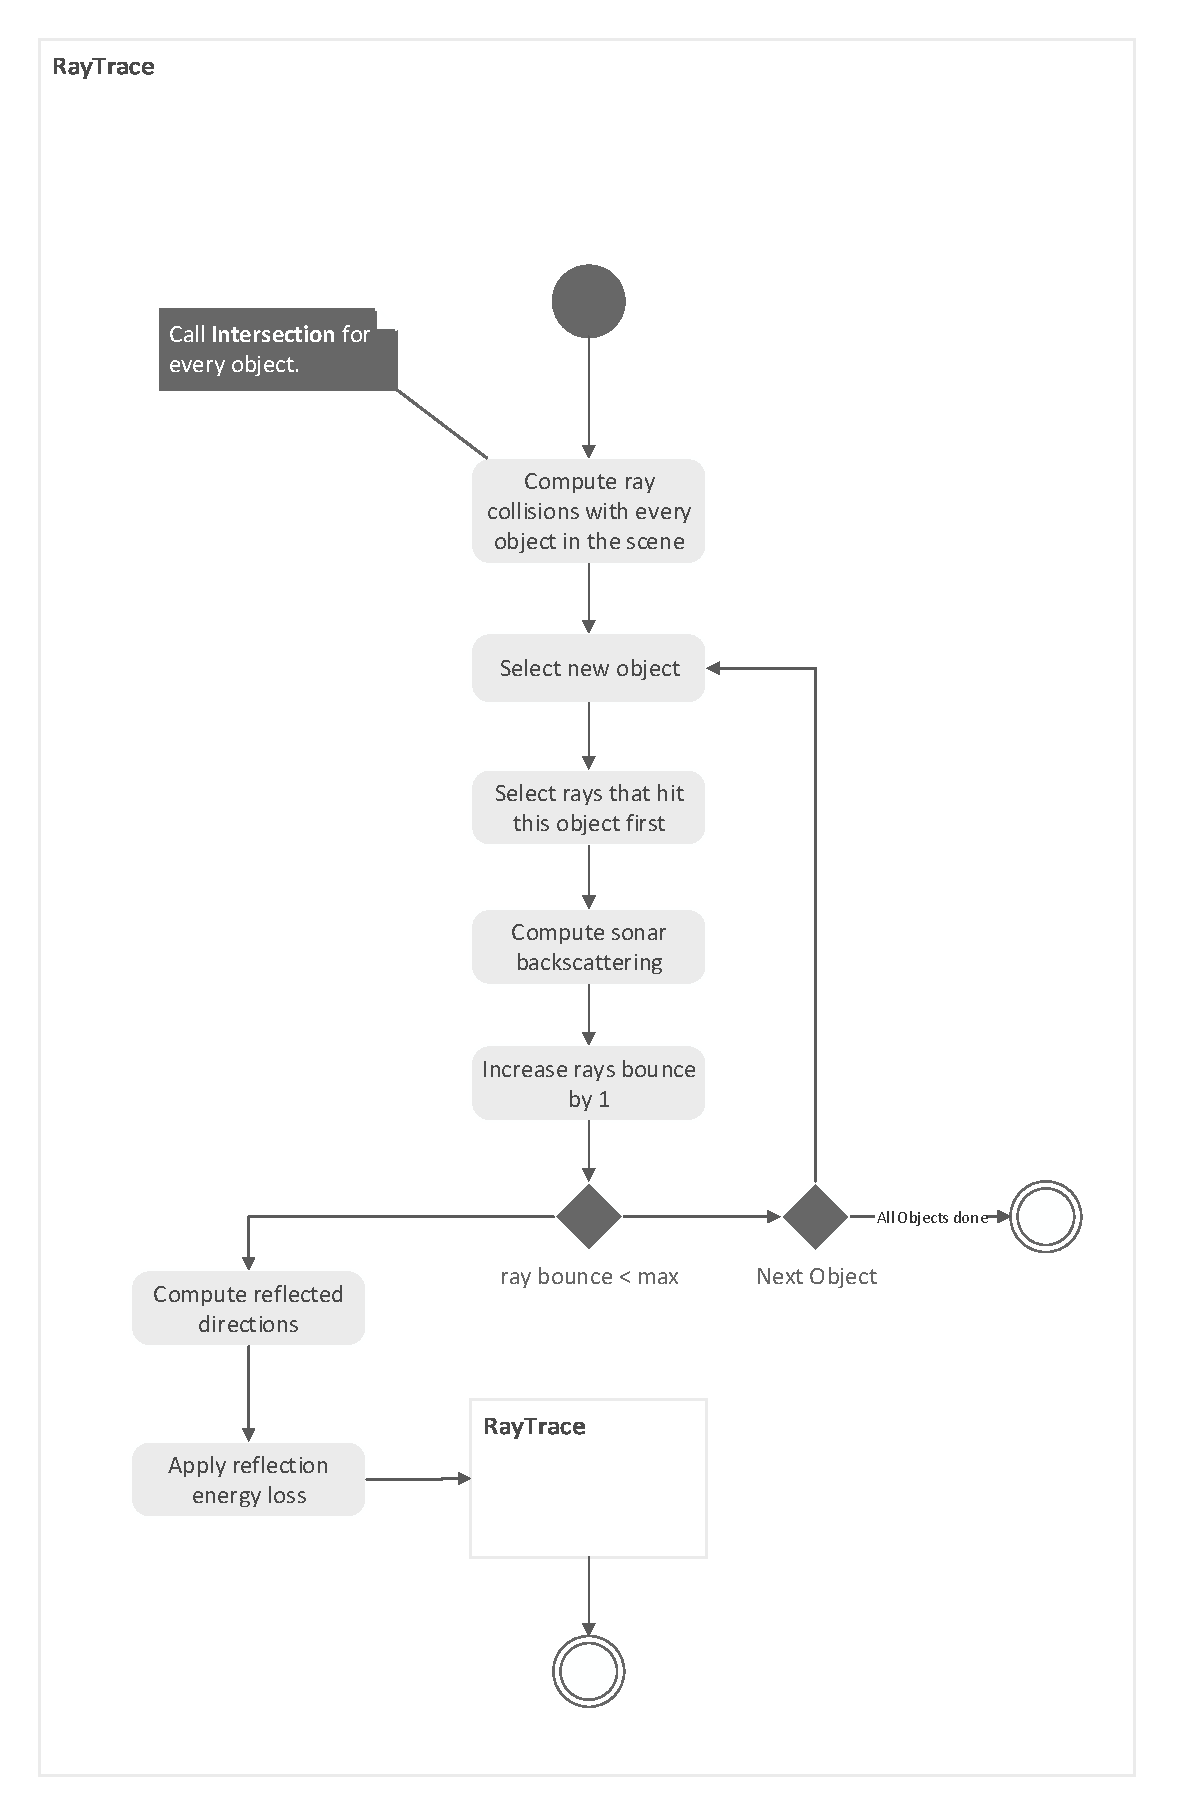
\includegraphics[width=75mm]{Chap2/fig/raytraceflow}}}%
    \caption{Overview of the simulation algorithm.}%
    \label{fig:algorithm}%
\end{figure}

Flowchart of figure \ref{fig:algorithm} describes the simulator logic. It starts
by computing ray directions spread over a sphere centered at the sonar with
uniform density, otherwise it would bias the ray trace. Not all directions are
actually computed because some directions have very low gain, so rays in these directions
have amost no energy, they can be discarted. To compute such a uniformly
distributed directions apply transformation described by algorithm
\ref{alg:urays} for $[-\alpha,\alpha]$ and $[-\beta,\beta]$ the vertical and
horizontal angular span, respectively, and $N$ the desired number of rays.
Results on section \ref{ss:results} use $\alpha = 30^o$ and $\beta = 3^o$,
approximatly the values for which Micron cannot detect the echo. 


\begin{algorithm}
\caption{Rays Uniform Direction}
\label{alg:urays}
\begin{algorithmic}
\Procedure{Uniform Direction}{$\alpha,\beta,N$}

\State $\dif\theta \gets 2\cos(\nicefrac{\pi}{2}-\alpha)$
\State $\dif\phi \gets 2\beta $
\State $\rho \gets \sqrt{\frac{N}{\dif\phi\cdot\dif\theta}}$ \Comment{Estimated
density}
\State $N_\theta \gets \lceil\rho\cdot\dif\theta\rceil$
\State $N_\phi \gets \lceil\rho\cdot\dif\phi\rceil$
\Comment{$U(\coord{x})$ generates $\coord{x}$ uniform samples over $[0,1]$}
\State $\theta \gets \arccos(\dif\theta\cdot (2U(N_\theta)-1))$ 
\State $\phi \gets \dif\phi\cdot (2U(N_\phi)-1)$

\ForAll{$(\theta_i,\phi_i) \in \theta\times\phi$}
\State $x_i \gets \sin(\theta_i)\cos(\phi_i)$
\State $y_i \gets \sin(\theta_i)\sin(\phi_i)$
\State $z_i \gets \cos(\theta_i)$
\State $v_i \gets (x_i,y_i,z_i)$
\EndFor

\State \textbf{return} $v$
\EndProcedure
\end{algorithmic}
\end{algorithm}

The sonar bearing pace is adjutable and, following Tritech's Micron
configuration, it was set to $1.8^o$, thus, doing a complete scan on $200$ steps. For each step, ray
directions are changed (by a rotation) to match new bearing. Received gain is
calculated w.r.t. the front direction (bearing), as the bearing changes the gain
is automatically updated. Rays aways carry 2 informations: its actual
intensity (disregaring distance traveled decay) and its total traveled length.

A new bearing position invoke ray tracer algorithm. It begins by calling
the \textbf{intersection} function (described at section \ref{ss:modeling}) for each
object in the scene, passing all rays as argument. Then it loops again on every
object, but now only focus on the rays that have the object as first hit, and
compute the backscattering to the sonar. Backscattering strength calculation use
Lambert and Phong scatterings as described on section \ref{sss:rays} and material
parameters listed on section \ref{ss:characterization}. This strength is add to
a bin (see figure \ref{fig:bins}) whose position is calculated as half the full
distance travelled by the ray (including previous reflections) plus a small
gaussian noise. It proceeds to calculate reflection if the number of computed
reflection for the ray does not exceed a maximum value (set to 5). Reflection
are simple linear transformations that depends on the surface's normal, obtained
via \textbf{normal} function (section \ref{ss:modeling}). The algorithm,then,
calls itself for the reflected rays, recursively.

After the whole scan is computed, bin values are normalized to $[0,\ldots,255]$
(again according to Tritech's Micron configuration ). Upon these values, an
additional Weibull's distributed noise is applied \cite{maussang2007mean}.

\subsection{Results}
\label{ss:results}

For both environments discribed on section \ref{ss:modeling}, several sonar
positions were simulated. The absolute position and orientation were chosen, but
the bearing w.r.t. the environment was a random value.

Polar plots displayed here is the expected visualization, without noise
filtering, when the sonar uses 500 bins of resolution with a 12 meters range.
Each polar pixel has a $3^o$ arc length, but, as the bearing step is $1.8^o$,
they overlap while being rendered.

\begin{figure}[ht]
    \centering \subfloat[Position $(0,0,0)$ | Orientation
    $(1,0,0)$]{{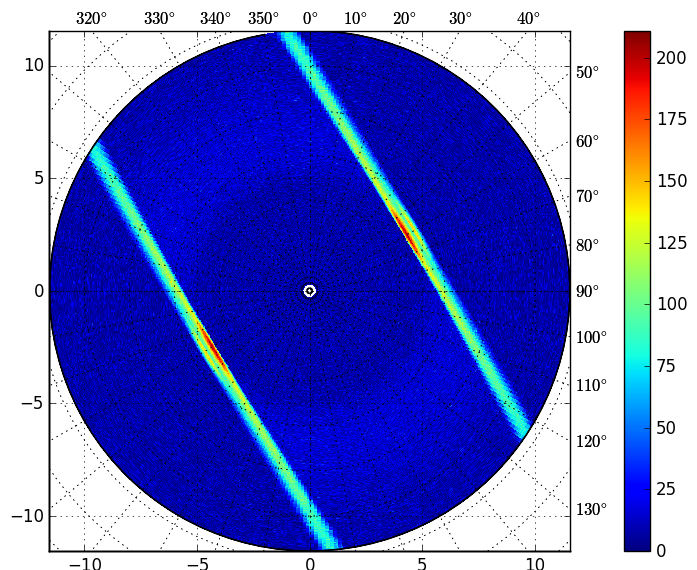
\includegraphics[width=75mm]{Chap2/fig/main_script__4_02_09_57_0,0,0_1,0,0f2}}}%
    \hfill \subfloat[Position $(0,0,6)$ | Orientation
    $(1,0,0)$]{{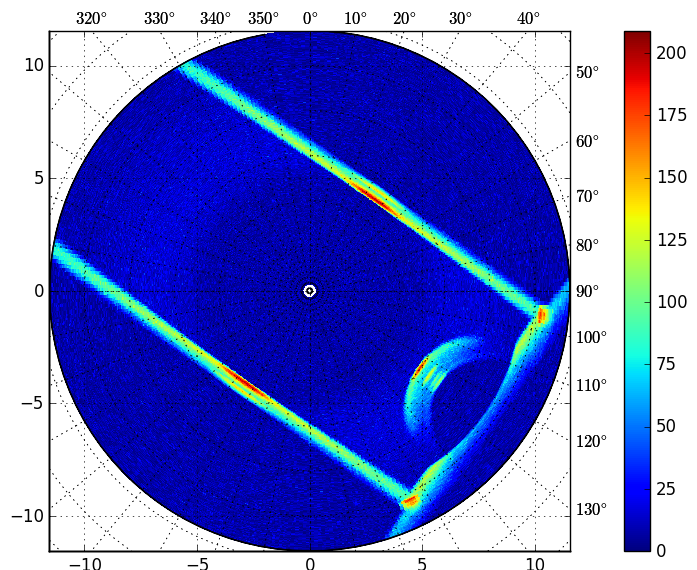
\includegraphics[width=75mm]{Chap2/fig/main_script__4_02_10_19_0,0,6_1,0,0f2}}}%
    \\
    \subfloat[Position $(-5,0,12)$ | Orientation
    $(0,1,0)$]{{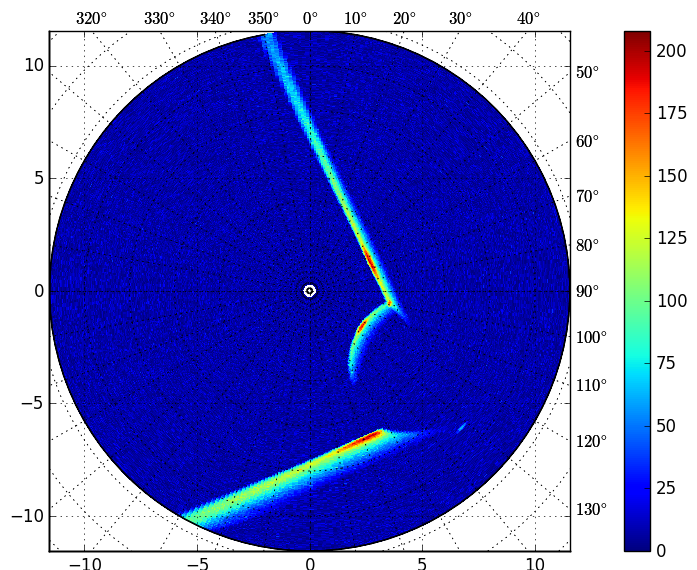
\includegraphics[width=75mm]{Chap2/fig/main_script__4_02_16_13_-5,0,12_0,1,0f2}}}%
    \hfill \subfloat[Position $(-5,0,12)$ | Orientation
    $(0,0,1)$]{{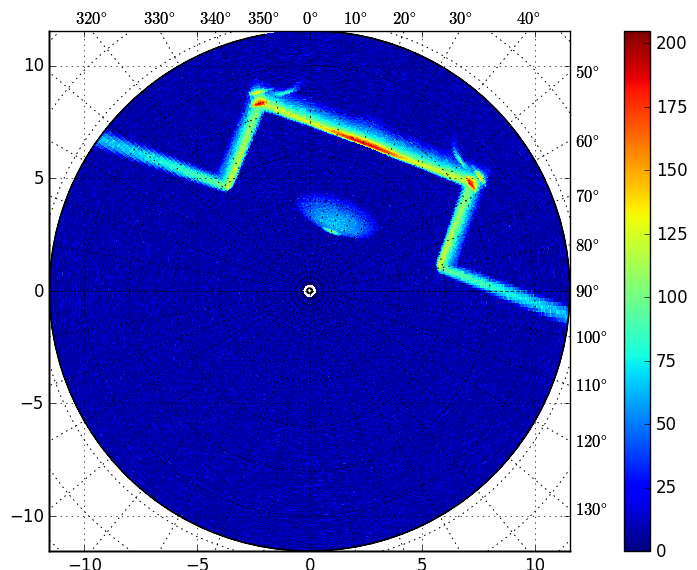
\includegraphics[width=75mm]{Chap2/fig/main_script__4_02_21_25_-5,0,12_0,0,1f2}}}%
    \caption{Sonar simulation for the complex scene.}%
    \label{fig:jirau_simul}%
\end{figure}


\begin{figure}[ht]
    \centering \subfloat[Position $(0,0,0)$ | Orientation
    $(1,0,0)$]{{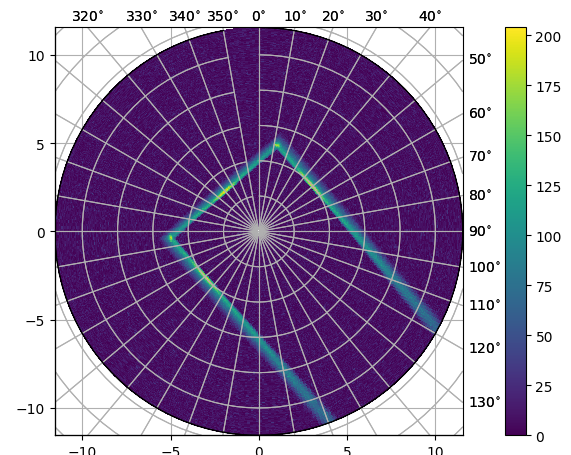
\includegraphics[width=75mm]{Chap2/fig/main_script__4_13_57_42_0,0,0_1,0,0f2}}}%
    \hfill \subfloat[Position $(4,1,0)$ | Orientation
    $(0,1,0)$]{{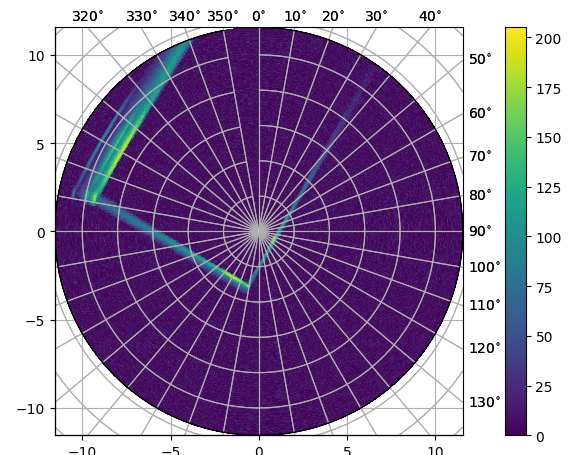
\includegraphics[width=75mm]{Chap2/fig/main_script__4_14_12_04_4,1,0_0,1,0f2}}}%
    \\
    \subfloat[Position $(0,0,0)$ | Orientation
    $(0,0,1)$]{{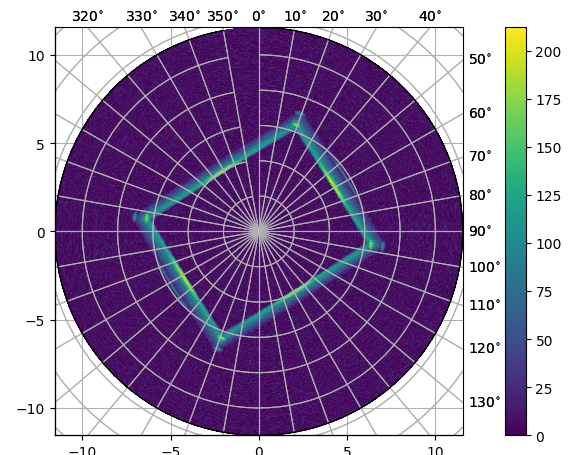
\includegraphics[width=75mm]{Chap2/fig/main_script__4_14_14_06_0,0,0_0,0,1f2}}}%
    \hfill \subfloat[Position $(0,3,0)$ | Orientation
    $(0,0,1)$]{{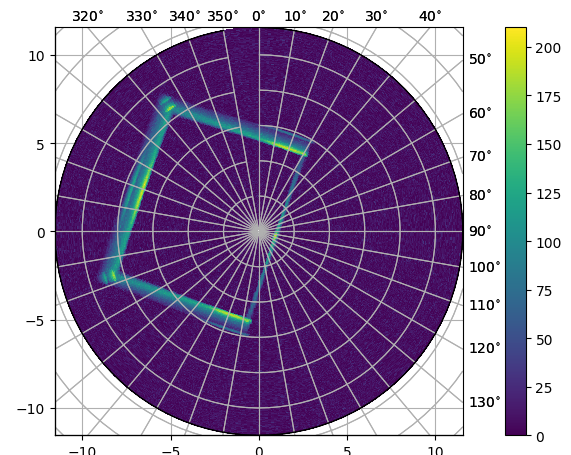
\includegraphics[width=75mm]{Chap2/fig/main_script__4_14_18_20_0,3,0_0,0,1f2}}}%
    \caption{Sonar simulation for the box-like scene.}%
    \label{fig:box_simul}%
\end{figure}
